\section{Used Models}
\label{sec:used_models}

\begin{figure}[h]
  \centering
  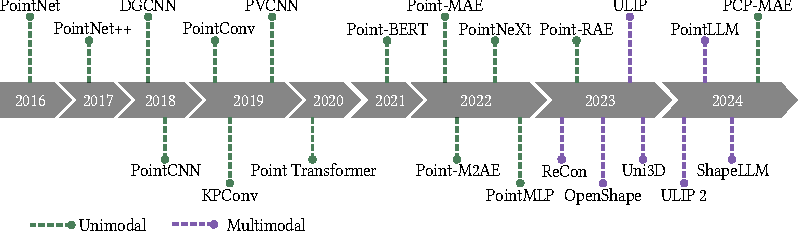
\includegraphics[width=1.0\linewidth]{figs/timeline.pdf}
  \caption{\textbf{Timeline of models used as 3D point-cloud encoders}}
  \label{fig:timeline}
\end{figure}

This section provides an extensive description of the models used in our experiments. We focused on three main types of models: point cloud-based models, transformer-based models, and persistence-based models. Since the latter require background on persistence homology, they're further detailed in Section~\ref{ssec:ph}. On the one hand, point cloud-based models are used as baselines for specific tasks (see Table~\ref{tab:topogen-results}). This choice stems from the widely known limitations in terms of robustness to input corruption and generalization~\cite{set-transformer} of such models. On the other hand, transformers have demonstrated state-of-the-art performance on various 3D shape understanding tasks~\cite{pbert,pmae,pm2ae,pcpmae}, and we are therefore insterested here in their ability to learn rich representations from data. 

\subsection{Baselines Models}
\label{ssec:baselines_models} 

We compare results obtained with transformer-based models to several baselines widely used in the literature. These models directly act on individual points without any tokenization step. They are all invariant to point permutations and can handle varying point cloud sizes. A final feature vector is obtained through a global pooling operation, which is then used for downstream tasks.

\subsubsection{PointNet}

PointNet~\cite{pointnet} introduced the first deep learning architecture that operates directly on raw 3D points. Each point is independently transformed through shared multilayer perceptrons (MLPs) to extract per-point features, which are then aggregated using a symmetric pooling function—typically max pooling—to obtain a global shape descriptor. This design ensures invariance to input permutation and robustness to geometric transformations through a learned spatial transformer network. However, since PointNet treats each point independently before pooling, it lacks the ability to explicitly capture local geometric structures and neighborhood relations within the point cloud.

\subsubsection{PointNet++}

PointNet++~\cite{pointnet++} extends PointNet by introducing a hierarchical feature learning mechanism that captures local geometric patterns at multiple scales. It partitions the point cloud into overlapping local regions using sampling and grouping operations, applies PointNet within each region to extract local features, and recursively aggregates them to form higher-level representations. This hierarchical structure allows PointNet++ to model fine-grained local geometry while maintaining the permutation invariance of PointNet. The introduction of radius-based grouping and multi-scale feature extraction significantly improves robustness to non-uniform sampling and enhances generalization to complex shapes.

\subsubsection{DGCNN (Dynamic Graph CNN)}

DGCNN~\cite{dgcnn} further advances local structure modeling by representing the point cloud as a dynamic graph, where edges connect each point to its k-nearest neighbors in the feature space. Unlike PointNet++’s static grouping, DGCNN updates the neighborhood graph at each layer, allowing feature dependencies to evolve adaptively as the representation becomes more abstract. The model applies an edge convolution operator that learns features based on both point attributes and relative positional differences, effectively capturing local geometric relations and contextual information. This dynamic graph formulation enables DGCNN to achieve strong performance on tasks requiring fine spatial reasoning, such as segmentation and shape classification. Even though earlier but also some recent models~\cite{pointcnn, pointconv, kpconv, pvcnn} have shown competitive performance, it is admitted that performance on DGCNN account for all the other possible baselines.

\subsection{Transformer-based Models}
\label{ssec:transformer_based_models}

\begin{figure}[h]
  \centering
  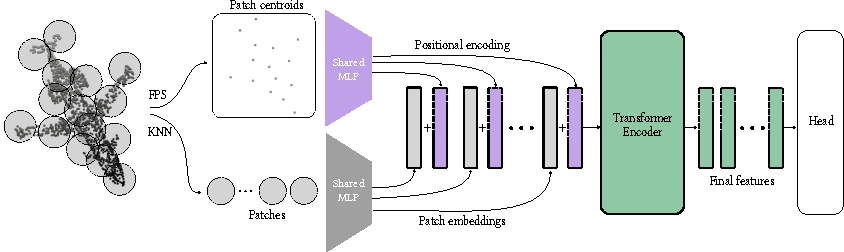
\includegraphics[width=1.0\linewidth]{figs/transformer_overview.pdf}
   \caption{\textbf{Transformer Overview for 3D point-clouds.} A point cloud is first partitioned into local patches using farthest point sampling (FPS) and K nearest neighbors (KNN). Patches are then embedded and augmented with positional encodings. The resulting sequence of patch embeddings is processed by a Transformer encoder to produce a global shape representation.}
   \label{fig:transformer-overview}
\end{figure}

Recent advances in transformer architectures for 3D shape understanding have largely built on the intuition that ideas from NLP and vision can be transferred to point cloud data. While the geometry of 3D shapes is fundamentally different from text or images, most models share a similar formal structure that follows three main stages: patchification, embedding, and token processing through a transformer encoder.

Let a point cloud be represented as a set of $N$ points: 
\begin{equation}
    \mathcal{P}=\{p_i \in \mathbb{R}^3\}_{i=1}^N.
\end{equation}

The patchification step partitions $\mathcal{P}$ into $M$ local regions $\{ \mathcal{P}_j \}_{j=1}^{M}$, each containing $K$ points. A common approach is to apply Farthest Point Sampling (FPS) to select $M$ center points $\{ \mathbf{c}_j \}_{j=1}^{M}$, and then group each center with its $K$ nearest neighbors using KNN:
\begin{equation}
    \mathbf{c}_j = \text{FPS}(\mathcal{P}), \quad \mathcal{P}_j = \text{KNN}(\mathbf{c}_j, \mathcal{P}) = \{p_{j,1},\dots,p_{j,K}\} \subset \mathbb{R}^3.
\end{equation}
Each patch $\mathcal{P}_j$ is thus a small local subcloud capturing fine-scale geometry around $\mathbf{c}_j$.

A lightweight local encoder $f_{\text{loc}}$ (often a PointNet variant) maps each patch to a feature vector:
\begin{equation}
    \mathbf{x}_j = f_{\text{loc}}(\mathcal{P}_j) \in \mathbb{R}^d,
\end{equation}

This produces a sequence of patch embeddings $\mathbf{X} = [\mathbf{x}_1, \dots, \mathbf{x}_M]^{\top} \in \mathbb{R}^{M \times d}$, which serves as the input to the transformer. The embedding dimension $d$ is fixed for all patches.

To provide geometric context, positional encodings are added to the embeddings. Each patch center $\mathbf{c}j$ is projected through a multilayer perceptron $f{\text{pos}}$:

\begin{equation}
  \mathbf{p}_j^\text{pos} = f_{\text{pos}}(\mathbf{c}_j) \in \mathbb{R}^d,
\end{equation}

The final input tokens are obtained as

\begin{equation}
  \mathbf{z}_j^{(0)} = \mathbf{x}_j + \mathbf{p}_j^\text{pos}
\end{equation}

Optionally, a learnable global token $\mathbf{z}_{\text{cls}}^{(0)} \in \mathbb{R}^{d}$ is prepended to the sequence to aggregate global information, yielding:

\begin{equation}
  \mathbf{Z}^{(0)} = [\mathbf{z}_{\text{cls}}^{(0)}; \mathbf{z}_1^{(0)}, \dots, \mathbf{z}_M^{(0)}] \in \mathbb{R}^{(M+1) \times d}.
\end{equation}

The transformer encoder then applies a stack of $L$ layers, each composed of multi-head self-attention (MSA) and feed-forward networks (FFN):

\begin{equation}
  \mathbf{Z}^{(l+1)} = \text{FFN}(\text{MSA}(\mathbf{Z}^{(l)})) + \mathbf{Z}^{(l)}, \quad l=0,\dots,L-1.
\end{equation}

The final output $\mathbf{Z}^{(L)}$ contains contextualized representations of all patches, where each token attends to others to model long-range dependencies across the shape. The representation of the class token $\mathbf{z}_{\text{cls}}^{(L)}$ (if used) or a global pooling of patch embeddings is then employed as the final shape descriptor.

This framework mirrors the architecture of Vision Transformers, with the key difference that the tokens correspond to irregular geometric neighborhoods rather than fixed image patches. Most recent models differ only in how the tokens are defined, how positional encodings are implemented, and what self-supervised pretraining objectives are used. These design variations lead to distinct inductive biases and training dynamics, as detailed in the following subsections.
% To preserve spatial structure, positional encodings are added by projecting the coordinates of the patch centers through an MLP, which provides the transformer with a notion of relative geometry between patches. The resulting sequence of patch embeddings, optionally augmented with a learnable global "class token" is then fed into a Transformer encoder. This process is conceptually identical to Vision Transformers, where image patches are tokenized, embedded, and processed sequentially, though here the tokens correspond to irregular geometric neighborhoods rather than regular image patches.

% This generic framework has provided the foundation for several influential works that differ primarily in how tokens are defined, how self-supervised pretraining is formulated, and whether hierarchical representations are incorporated. We now discuss these paradigms in detail.

\subsubsection{Point-BERT: Discrete Tokenization and Masked Modeling}
\label{sssec:pointbert}

Point-BERT~\cite{pbert} was among the first methods to transfer the BERT-style masked pretraining paradigm to point clouds. Its core idea is to convert each patch embedding $\mathbf{x}_j \in \mathbb{R}^d$ into a discrete token index, enabling the use of a masked language modeling objective analogous to NLP.

To achieve this, a discrete variational autoencoder (dVAE) is first trained to quantize the continuous patch embeddings. The encoder of the dVAE, $f_{\text{enc}}^{\text{dVAE}}$, maps a patch $\mathcal{P}_j$ to a latent code:

\begin{equation}
    \mathbf{h}_j = f_{\text{enc}}^{\text{dVAE}}(\mathcal{P}_j) \in \mathbb{R}^{d'}
\end{equation}

This latent code is then discretized by assigning it to its nearest entry in a learnable codebook $\mathcal{C} = { \mathbf{c}1, \dots, \mathbf{c}{|\mathcal{C}|} } \subset \mathbb{R}^d$:

\begin{equation}
    \tilde{\mathbf{h}}_j = \mathbf{c}_{k_j}, k_j = \arg\min_{k} || \mathbf{h}_j - \mathbf{c}_k ||_2
\end{equation}

The decoder $f_{\text{dec}}^{\text{dVAE}}$ reconstructs the original patch from $\tilde{\mathbf{h}}_j$, ensuring that each codeword captures meaningful local geometry.

Once the vocabulary is trained, the transformer is pretrained with Masked Point Modeling (MPM). A subset $\mathcal{M} \subset {1, \dots, M}$ of patches is masked, and the model receives as input only the unmasked tokens and their positional encodings. The objective is to predict the discrete indices ${k_j}_{j \in \mathcal{M}}$ of the masked patches:

\begin{equation}
    \mathcal{L}_{\text{MPM}} = - \sum_{j \in \mathcal{M}} \log p_\theta(k_j | \{\mathbf{z}_i^{(0)}\}_{i \notin \mathcal{M}})
\end{equation}

where $p_\theta$ is parameterized by the transformer. A learnable global token $\mathbf{z}_{\text{cls}}^{(0)}$ is updated jointly with the patch tokens during pretraining, and its final state $\mathbf{z}_{\text{cls}}^{(L)}$ is used as the shape embedding for downstream tasks.


\subsubsection{Point-MAE: Continuous Tokens and Masked Autoencoding}
\label{sssec:pointmae}

Point-MAE~\cite{pmae} simplifies this framework by removing discrete tokenization and operating directly on continuous patch embeddings. Each patch $\mathcal{P}_j$ is encoded as a continuous vector $\mathbf{x}_j = f_{\text{loc}}(\mathcal{P}_j) \in \mathbb{R}^{d}$, and a random subset $\mathcal{M}$ of them is masked. Only the unmasked patches are passed to the transformer encoder.

A shared learnable vector $\mathbf{t}_{\text{mask}} \in \mathbb{R}^d$ replaces the embeddings of masked patches. The transformer encoder processes only unmasked embeddings:

\begin{equation}
  \mathbf{Z}_\text{enc}=\text{Encoder}(\{\text{x}_j+p_j^\text{pos}\}_{j \notin \mathcal{M}})
\end{equation}

Then a lightweight decoder reconstructs the masked patches from the concatenation of encoder outputs and mask tokens:

\begin{equation}
  \mathbf{Z}_\text{dec}=\text{Decoder}([\mathbf{Z}_\text{enc}; \{\mathbf{t}_{\text{mask}}+p_j^\text{pos}\}_{j \in \mathcal{M}}])
\end{equation}

The reconstruction target is the set of 3D coordinates ${\mathcal{P}_j}{j \in \mathcal{M}}$, and the loss is usually a Chamfer distance:
\begin{equation}
  \mathcal{L}_{\text{MAE}} = \sum_{j \in \mathcal{M}} \text{Chamfer}(\hat{\mathcal{P}}_j, \mathcal{P}_j)
\end{equation}

This continuous formulation avoids the need for a pretrained tokenizer and allows more efficient computation since only unmasked patches go through the heavy encoder. It also directly learns a geometric reconstruction objective rather than a discrete prediction one. Unlike Point-BERT, the class token is not used during pretraining but introduced only during fine-tuning for downstream tasks. This makes pretraining focus on local geometric recovery, leaving semantic aggregation to task-specific adaptation.

\subsubsection{Hierarchical Extensions: Multi-Scale Representations}
\label{sssec:hierarchical_extensions}

Point-M2AE~\cite{pm2ae} extends Point-MAE by introducing multi-scale feature processing to better capture hierarchical shape structure. Given the initial point cloud $\mathcal{P}$, successive downsampling layers produce coarser point sets $\mathcal{P}^{(1)}, \mathcal{P}^{(2)}, \dots$, with decreasing sizes $N_1 > N_2 > \dots$ and corresponding patch sets $\{ \mathcal{P}^{(\ell)}_j \}_{j=1}^{M_\ell}$. Each scale has its own embedding function $f_{\text{loc}}^{(\ell)}$, producing patch features $\mathbf{X}^{(\ell)} \in \mathbb{R}^{M_\ell \times d_\ell}$.

\begin{equation}
  \mathbf{Z}^{(\ell+1)} = \text{Transformer}^{(\ell)}(\mathbf{X}^{(\ell)},\mathbf{Z}^{(\ell-1)})
\end{equation}

This design parallels the feature hierarchies in PointNet++ and U-Net architectures, allowing Point-M2AE to represent both fine-grained details and global context. The masking strategy is also applied at multiple scales to ensure consistency across abstraction levels.

By combining local spatial self-attention at fine resolutions with global aggregation at coarser ones, Point-M2AE improves generalization and compactness, outperforming single-scale variants on both classification and reconstruction tasks.

\subsubsection{Further Improvements}
\label{sssec:further_improvements}

Several recent works refine the MAE framework to better encode geometric priors and invariances.
PCP-MAE~\cite{pcpmae} modifies positional encodings to prevent information leakage: instead of directly providing patch centers $\mathbf{c}_j$, it requires the model to predict them, forcing reliance on relational geometry rather than absolute positions.
HFBRI-MAE~\cite{hfbrimae} augments each token with handcrafted rotation-invariant descriptors, ensuring robustness to arbitrary 3D rotations.
Point-RAE~\cite{prae} introduces a regression-before-autoencoding strategy, first predicting geometric features and then reconstructing points. This separation decouples encoder and decoder learning, preventing overfitting of the reconstruction loss.

Together, these improvements show that incorporating geometric inductive biases into the transformer pipeline strengthens both robustness and generalization.

\subsubsection{Comparative View}
\label{sssec:comparative_view}

Despite architectural differences, all transformer-based 3D encoders share the same formal backbone described by Figure~\ref{fig:transformer-overview}. They differ mainly in how tokens are defined (discrete vs. continuous), the pretraining objective (classification vs. reconstruction), and the presence of hierarchical processing.

Point-BERT’s discrete modeling brings a language-like structure but requires a learned tokenizer.\\
Point-MAE simplifies the pipeline and enables efficient continuous pretraining.\\
Point-M2AE extends this formulation to multiple scales, encoding richer geometric dependencies.

This report focuses on Point-BERT, Point-MAE, and Point-M2AE as representative models, as they capture the main design paradigms in transformer-based 3D shape understanding. It also considers PCP-MAE as it builds directly on Point-MAE and is the current state-of-the-art on most downstream tasks we further describe.

% Despite their differences, Point-BERT, Point-MAE, and their hierarchical successors share a common foundation: the adaptation of the transformer paradigm from language and vision to point clouds through \textit{patchification}, embedding, and positional encoding. What distinguishes them is how tokens are defined, how the self-supervised objective is formulated, and whether hierarchical geometry is explicitly modeled. Discrete-token approaches like Point-BERT require a two-stage pretraining pipeline but tightly align with NLP pretraining paradigms. Continuous-token methods like Point-MAE are simpler and more efficient, emphasizing reconstruction over classification. Hierarchical extensions such as Point-M2AE incorporate multiscale representations, bringing additional inductive structure into the transformer.

% An important consequence of these differences is that evaluation protocols vary across models. Point-BERT pretraining relies on predicting discrete token IDs, while Point-MAE and M2AE use reconstruction losses such as Chamfer distance. The role of the CLS token also differs, being central during pretraining in Point-BERT but absent in MAE-style approaches. As a result, downstream fine-tuning and linear probing must be carefully adapted to each architecture. The precise evaluation settings for each method will be detailed in the following experimental section.

\subsection{Multimodal approaches}
\label{ssec:multimodal}

Several recent works extend 3D transformers to multimodal settings by aligning point cloud embeddings with image and text features in a shared latent space. Given a 3D encoder $f_{\text{3D}}$ producing embeddings $\mathbf{z}_{\text{3D}} \in \mathbb{R}^d$, and pretrained encoders $f_{\text{img}}$, $f_{\text{text}}$, the goal is to enforce semantic consistency through a contrastive objective:

\begin{equation}
  \mathcal{L}_{\text{align}} = 
  - \log 
  \frac{
    \exp\left(\text{sim}(\mathbf{z}_{\text{3D}}, \mathbf{z}_{\text{img}}) / \tau\right)
  }{
    \sum_{(\mathbf{z}'_{\text{3D}}, \mathbf{z}'_{\text{img}})}
    \exp\left(\text{sim}(\mathbf{z}'_{\text{3D}}, \mathbf{z}'_{\text{img}}) / \tau\right)
  }.
\end{equation}


where $\text{sim}$ denotes cosine similarity.

ULIP~\cite{ulip} and ULIP-2~\cite{ulip2} follow this strategy by coupling Point-BERT with image and text encoders. The resulting models learn cross-modal alignment but remain bounded by the geometric expressiveness of the 3D backbone. PointLLM~\cite{pointllm} further connects a frozen 3D encoder to a large language model through a lightweight adapter, while ShapeLLM~\cite{shapellm} and Uni3D~\cite{uni3d} generalize the same principle using multi-view or ViT-based 3D encoders.

Although these systems broaden the representational scope of 3D models, their effectiveness strongly depends on the unimodal encoder. The quality of $\mathbf{z}_{\text{3D}}$ determines how well multimodal alignment preserves geometric structure. Our own trials confirmed that replacing or fine-tuning the multimodal layers rarely compensates for weaknesses in the 3D representation itself.

\paragraph{Why we focus on unimodal encoders.}
Because multimodal models inherit the inductive biases of their 3D backbones, we restrict our analysis to unimodal encoders. This allows us to isolate how transformers process geometric and topological structure within point clouds, without interference from external modalities. In Section~\ref{sec:experiments}, we further quantify how such encoders capture non-semantic information using persistence-based analysis.

% A number of recent works couple 3D encoders with images and text. ULIP~\cite{ulip} aligns point clouds, images, and text in a shared space. In practice it uses Point-BERT as the 3D encoder, and reports results directly with that backbone. ULIP-2~\cite{ulip2} scales the same idea with generated captions and larger backbones. Its main 3D backbones are Point-BERT and PointNeXt~\cite{pointnext}, with Point-BERT remaining a primary option throughout the study.

% PointLLM~\cite{pointllm} connects a frozen point cloud encoder to a language model through a small projector and performs alignment then instruction tuning. The paper states that Point-BERT pretrained with ULIP-2 serves as the point encoder. ShapeLLM~\cite{shapellm} targets embodied interaction with a dedicated encoder named ReCon++. The authors build ReCon++ by multi view distillation and use it as the base 3D representation before instruction tuning, rather than Point-BERT or Point-MAE.

% ReCon~\cite{recon} itself is a pretraining framework that mixes generative reconstruction with contrastive learning. It supports single modality and cross modality inputs and can use cross modal teachers. It is not tied to Point-BERT or Point-MAE although comparisons to both are reported. Uni3D~\cite{uni3d} scales a ViT style backbone to 3D and aligns 3D point features to image text features with 2D initialized weights. It does not rely on Point-BERT or Point-MAE.

% Taken together, many multimodal systems still depend on the quality of the 3D encoder and often choose Point-BERT. ULIP and PointLLM are explicit examples. ShapeLLM and Uni3D move away from Point-BERT and Point-MAE but remain bounded by 3D encoder design choices. This observation is central to the scope of our study.

% \paragraph{Why we focus on unimodal encoders.} Because multimodal models inherit the inductive biases of their 3D backbones, we restrict our analysis to unimodal encoders. This allows us to isolate how transformers process geometric and topological structure within point clouds, without interference from external modalities. In Section~\ref{ssec:ph}, we further quantify how such encoders capture non-semantic information using persistence-based analysis.